\documentclass{beamer}
\usetheme{default} % You can swap theme if you like (e.g., Madrid, Boadilla)
\usepackage{tikz} 



\title{Starter: Expanding Brackets}
\author{Year 8}
\date{}

\begin{document}

\begin{frame}
  \titlepage
\end{frame}

% ---------- STARTER (2x2 layout) ----------
\begin{frame}{Starter: Expand each expression}
% Option A: simple 2x2 grid using minipages (consistent spacing)
\begin{minipage}[t]{0.48\textwidth}
  \begin{block}{1) Single brackets}
    \Large \( \;3(y+5) \)
  \end{block}
  \vspace{0.5em}
  \begin{block}{3) Double brackets}
    \Large \( \;(x+4)(x-2) \)
  \end{block}
\end{minipage}\hfill
\begin{minipage}[t]{0.48\textwidth}
  \begin{block}{2) Single brackets}
    \Large \( \; a(b-5)\)
  \end{block}
  \vspace{0.5em}
  \begin{block}{4) What is the area of the rectangle?}
    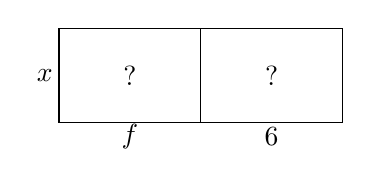
\begin{tikzpicture}[scale=0.6]

% Outer rectangle
\draw (0,0) rectangle (6,2);

% Vertical split
\draw (3,0) -- (3,2);

% Labels for widths
\node at (1.5,-0.3) {$f$};
\node at (4.5,-0.3) {$6$};

% Height label
\node at (-0.3,1) {$x$};

% Area labels
\node at (1.5,1) {?};
\node at (4.5,1) {?};

\end{tikzpicture}
  \end{block}
\end{minipage}
\end{frame}

% ---------- ANSWERS ----------
\begin{frame}{Answers}
\begin{enumerate}
  \item \(3(y+5)=3y+15\)
  \item \(a(b-5)=ab-5a\)
  \item \((x+4)(x-2)=x^2+2x-8\)
  \item Area = \(xf + 6x = x(f+6)\)
\end{enumerate}
\end{frame}

\end{document}